\documentclass[letterpaper]{article}
\usepackage{lindrew}
\usepackage{titling}
\usepackage{float}
\usepackage{subcaption}

\hypersetup{pdftitle={GitHub Analytics}, pdfauthor={Farhan Sadeek}}
\begin{document}
\title{\textbf{GitHub Analytics} \\ \Large Analyzing the GitHub Network}
\author{Farhan Sadeek}
\date{\today}

\maketitle
\tableofcontents
\newpage
\section{Abstract}
The objective of this project is to analyze the GitHub social network, gathered from the MUSAE project. The dataset contains 37,700 nodes, each representing developers who have starred at least ten repositories, and 289,003 undirected edges corresponding to mutual follower relationships. Each node is labeled as either a Machine Learning Engineer or a Web Developer, based on the individual's job title. This study will use graph analysis techniques to investigate the relationships within these graphs.
\section{Introduction}
\subsection{Motivation and Importance}
Since GitHub is the most popular platform for hosting and sharing open-source software \cite{hague2022globalgithub}, many computer programmers maintain a GitHub profile because it provides an accessible and cost-effective way to share code internationally. In professions such as Software Engineering and Data Science, recruiters and hiring managers often ask candidates for access to their GitHub profiles, viewing them as portfolios of publicly available projects.

\subsection{Prior Work in the same Field}
The dataset used in this study was part of the MUSAE project \cite{rozemberczki2021musae}, a collection of datasets from \href{https://snap.stanford.edu/data/github-social.html}{Stanford Network Analysis Project}. In the study, the authors introduced an attribute, MUSAE, for learning node embeddings. In this study, they demonstrated that the MUSAE method outperformed contemporary methods for node classification tasks \cite{rozemberczki2021musae}.

\subsection{Limitations}
There were several limitations to the dataset used for this study. First of all, this data is a snapshot of the developer community from June 2019, which might not reflect the reflect the contemporary shift towards Machine Learning, and will likely require updates in the near future to be more useful. Additionally, there are significantly more titles than just Machine Learning Engineer or Web Developer, so it's not the most ideal way to represent the data. Additionally, this network assumes that the relationship between two contributors is mutual. This means contributions to shared and public repositories, code reviews, and shared activities are not included, which is a key aspect of GitHub. Lastly, the minimum number of followers required to be included in this data is 10, which is large and might not be the most representative of the actual network.

\section{Data}
\subsection{Source and Creation}
The dataset used in this study was originally created as part of the MUSAE project and is currently hosted in the \href{https://snap.stanford.edu/data/github-social.html}{Stanford SNAP} collection \cite{snapnets}. The authors collected developer information using the GitHub API in June 2019 as part of their research project.

\subsection{About the Dataset}
Initial exploration of the data shows that this is a \textbf{simple}, \textbf{undirected}, \textbf{globally connected} network of $N = 37{,}700$ developers and $E = 289{,}003$ edges. In this network topology, nodes represent developers classified as either Web Developer or Machine Learning Engineer, and edges represent mutual follower relationships. The structural and attribute data for this network are split across two datasets: \texttt{musae\_git\_edgelist.csv}, which contains the edges, and \texttt{musae\_git\_attributes.csv}, which contains the node attributes.

\section{Methods}
Using the \texttt{igraph} package \cite{csardi2006igraph} in R, we constructed an undirected graph from the edgelist and confirmed it is a simple graph with no self-loops or multiple edges. Subsequently, following the methodology of Kolaczyk and Csardi~\cite{kolaczyk2020sand}, we analyzed this network to identify interesting graph properties and potential patterns in the data.

\subsection{Descriptive Analysis}
A descriptive analysis of this graph shows that it is \textbf{simple}, \textbf{connected}, \textbf{undirected}, comprises 37,700 nodes and 289,003 edges, and has a graph density of $4.07 \times 10^{-4}$.
\begin{table}[H]
  \centering
  \begin{tabular}{lrrrrrrrr}
    \toprule
    \textbf{Nodes} & \textbf{Edges} & \textbf{Density} & \textbf{Components} & \textbf{Diameter} & \textbf{Avg Path} & \textbf{Transitivity} & \textbf{Max $k$-core} \\
    \midrule
    37,700 & 289,003 & $4.07 \times 10^{-4}$ & 1 & 11 & 3.24 & 0.0124 & 34 \\
    \bottomrule
  \end{tabular}
  \caption{Global properties of the GitHub mutual-follower network.}
  \label{tab:global}
\end{table}

In this network, each node is classified as either a Web Developer or a Machine Learning Engineer, a binary classification for this project, unlike a bipartite graph. However, the nodes aren't completely different objects, as in the Netflix dataset, where movies and humans are two distinct node types. The nodes are classified as follows:
\begin{table}[H]
  \centering
  \begin{tabular}{|l|r|r|}
    \hline
    \textbf{Label} & \textbf{Count} & \textbf{Percent} \\
    \hline
    Web (0) & 27,961 & 74.2\% \\
    MLE (1) & 9,739 & 25.8\% \\
    \hline
  \end{tabular}
  \caption{Distribution of developer type labels in the MUSAE GitHub network}
\end{table}

Since this data dates back to 2019, it shows an interesting trend in modern software development. Because at that time, web developers (programmers who create websites) were in high demand. However, that landscape has changed significantly with the rise of Large Language Models. \cite{Upwork2026AIWebDev}

\subsection{Top Hub Nodes}
Looking at the 2019 data, it becomes clear that the most connected nodes are web developers, indicating the popularity of programming websites among both hobbyists and professionals, and the role \href{https://github.com}{GitHub} played at that time for builders. This is further confirmed by the presence of people like \textit{addyosmani}, former director of Chrome Development tools at Google, and \textit{jeresig}, the creator of jQuery, \textit{mdo}, co-creator of a popular web design framework Bootstrap, and \textit{kentcdodds}, a popular \href{https://react.dev}{React} developer and educator.
\begin{table}[H]
  \centering
  \begin{tabular}{rlrrr}
    \toprule
    \textbf{Rank} & \textbf{Developer} & \textbf{Node ID} & \textbf{Degree} & \textbf{Label} \\
    \midrule
    1  & dalinhuang99         & 31890 & 9,458 & Web \\
    2  & nfultz               & 27803 & 7,085 & Web \\
    3  & addyosmani           & 35773 & 3,324 & Web \\
    4  & Bunlong              & 19222 & 2,958 & Web \\
    5  & gabrielpconceicao    & 13638 & 2,468 & Web \\
    6  & rfthusn              & 36652 & 2,343 & Web \\
    7  & nelsonic             & 18163 & 1,924 & Web \\
    8  & getify               & 9051  & 1,797 & Web \\
    9  & mdo                  & 35008 & 1,571 & Web \\
    10 & ronenhamias          & 10001 & 1,568 & Web \\
    11 & SuriyaaKudoIsc       & 36628 & 1,507 & Web \\
    12 & jeresig              & 7027  & 1,485 & Web \\
    13 & JonnyBanana          & 19253 & 1,404 & Web \\
    14 & mbostock             & 2078  & 1,368 & Web \\
    15 & shayan-taheri        & 33671 & 1,347 & Web \\
    \bottomrule
  \end{tabular}
  \caption{Top 15 developers by mutual followers}
  \label{tab:top_hubs}
\end{table}

\subsection{Degree and Edge Distribution}
The degree and edge distribution tell us about the overall structure of the graph, such as the number of nodes and edges, the density of the graph, and the distribution of degrees among the nodes, which reveals if the network acts like a small world, and the sparsity, which might be useful for understanding the network better.
\begin{table}[H]
  \centering
  \begin{tabular}{|l|r|}
    \hline
    \textbf{Statistic} & \textbf{Degree} \\
    \hline
    Min    & 1 \\
    Q1     & 2 \\
    Median & 6 \\
    Mean   & 15.33 \\
    Q3     & 13 \\
    90th Percentile & 30 \\
    99th Percentile & 99 \\
    Max    & 9458 \\
    \hline
  \end{tabular}
  \caption{Degree distribution}
\end{table}
Since the median is almost 2.5 times smaller than the mean, it suggests that the degree distribution is skewed to the right, because of outliers. Similarly, the 90th percentile is 5 times the median, and the 99th percentile is 16 times the median, further confirming that the degree distribution is skewed to the right. The degree distribution in a logarithmic and linear chart is plotted below
\begin{figure}[H]
  \centering
  \begin{subfigure}[t]{0.48\textwidth}
    \centering
    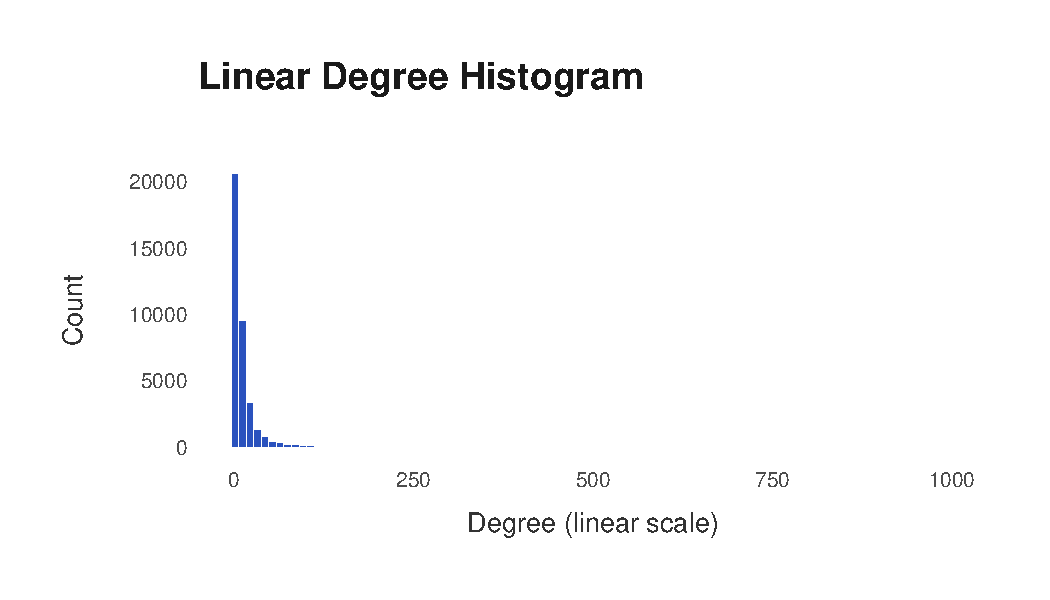
\includegraphics[width=\textwidth]{output_plots/linear_degree_histogram.pdf}
    \caption{Linear scale histogram}
    \label{fig:degree_linear}
  \end{subfigure}
  \hfill
  \begin{subfigure}[t]{0.48\textwidth}
    \centering
    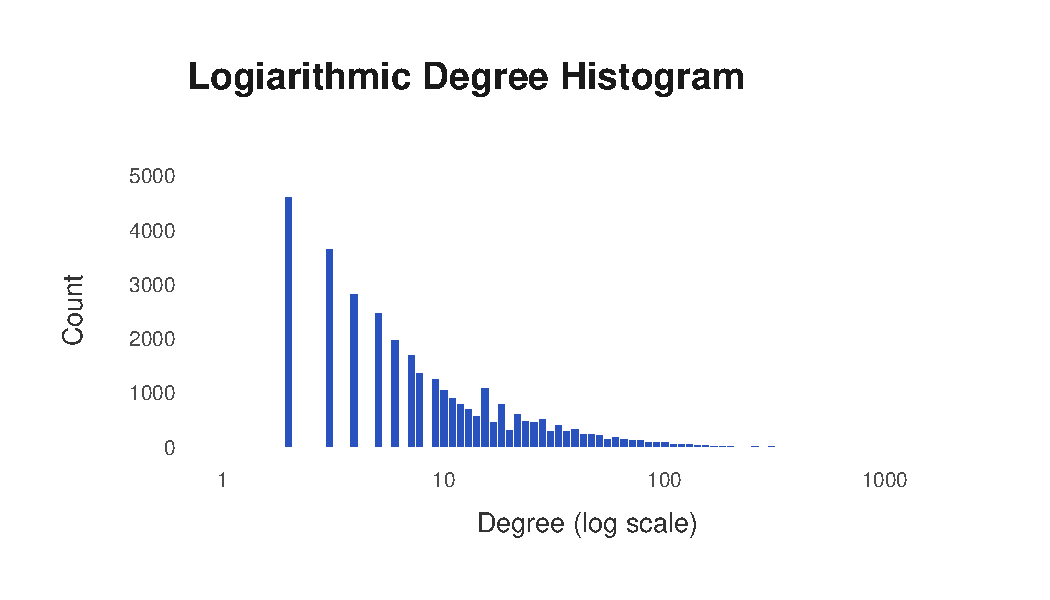
\includegraphics[width=\textwidth]{output_plots/log_log_degree_histogram.pdf}
    \caption{Log--log degree distribution}
    \label{fig:degree_loglog}
  \end{subfigure}
  \caption{Degree distribution of the GitHub network. The linear plot (a) highlights the massive concentration of low-degree nodes, while the log--log plot (b) indicates a potential power-law tail.}
  \label{fig:degree_comparison}
\end{figure}

From this log-log plot, it is clear that the degree distribution follows a power law, indicating that a few nodes are connected to most of the nodes in the network. This highlights an important structural feature: influential developers play a critical role in community connectivity, reinforcing the importance of network effects within GitHub.

\subsection{Vertex Centrality}
Vertex centrality measures the importance of individual nodes in a network \cite{freeman1978centrality}. For this project, four centrality measures were computed using functions available in the igraph package for R. Due to the network's size, it wasn't possible to plot the visualizations; the following analysis would provide strong evidence instead.

\begin{table}[H]
  \centering
  \caption{Summary Statistics of Network Centrality Measures}
  \begin{tabular}{l|rrrr}
    \hline
    Statistic & Degree & Betweenness & Closeness & Eigenvector \\
    \hline
    Minimum      & 0.00002653 & 0.000000001 & 0.1414 & 0.0000000 \\
    1st Quartile & 0.00005305 & 0.000000045 & 0.2841 & 0.0004698 \\
    Median       & 0.0001592  & 0.000001529 & 0.3113 & 0.0030462 \\
    Mean         & 0.0004067  & 0.000059592 & 0.3137 & 0.0066687 \\
    3rd Quartile & 0.0003448  & 0.000017282 & 0.3469 & 0.0089577 \\
    Maximum      & 0.2509689  & 0.269626963 & 0.5231 & 1.0000000 \\
    \hline
  \end{tabular}
\end{table}

Looking at the \textbf{degree centrality}, the maximum value (0.25) is about 600 times the mean value (0.0004067), which means that there are a few nodes that are connected to most of the nodes in the network. Furthermore, the \textbf{eigenvector centrality} has a maximum value of 1.0 and its mean is 0.0067, which means that not only are the very well-connected nodes connected to other nodes at random, but they are also connected to other nodes that are also very well-connected. Now for \textbf{betweenness centrality}, the maximum value is 0.270, and their mean is almost zero, which means that most nodes show minimal reachability and betweeenness. However, some nodes with extremely high betweenness centrality are bridges in the graph, meaning they connect different communities. These are the articulation points in a network from an economics perspective. Lastly, the \textbf{closeness centrality} has a maximum value of 0.5231, and its mean is 0.3137, which are relatively close to each other compared to the other ones, which implies that the network might be large, but it's very tight-knit.

\begin{figure}[H]
  \centering
  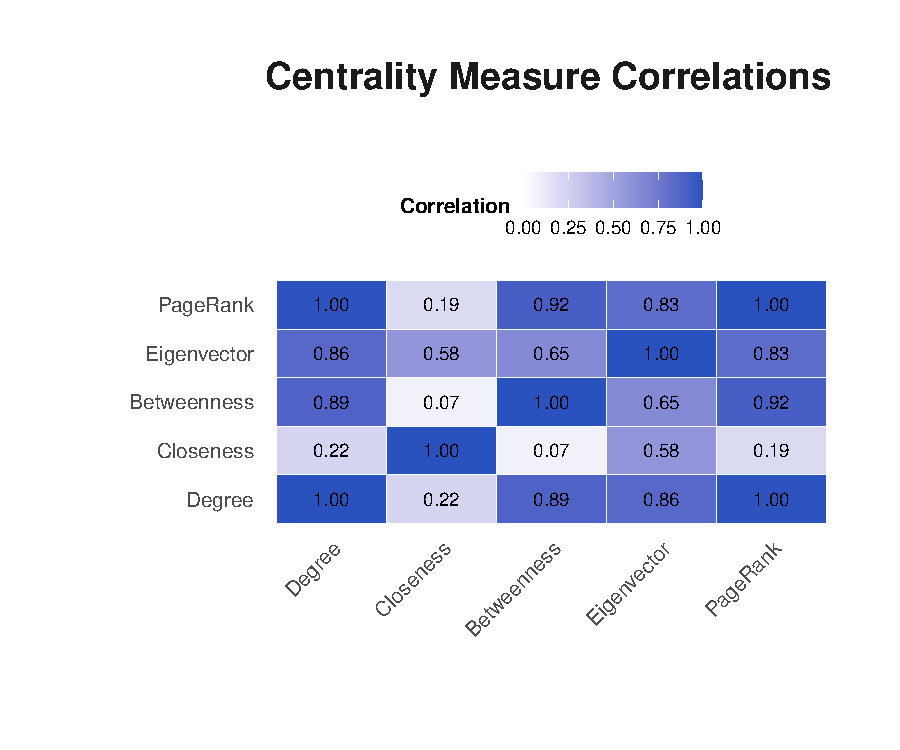
\includegraphics[width=0.8\textwidth]{output_plots/centrality_correlation.pdf}
  \caption{Correlation between centrality measures in the GitHub network}
  \label{fig:centrality_correlation}
\end{figure}

This correlation plot shows that most centrality measures are closely correlated with each other, except for betweenness centrality.

\subsection{Component Structure}
In this network, there is a single giant component that encompasses all nodes and edges.
\begin{table}[H]
  \centering
  \begin{tabular}{|c|c|c|c|}
    \hline
    \textbf{Components} & \textbf{Nodes} & \textbf{Edges} & \textbf{Articulation Points} \\
    \hline
    1 & 37,700 & 289,003 & 350 \\
    \hline
  \end{tabular}
  \caption{Properties of the giant component in the GitHub network.}
\end{table}

This network contains a single giant component, meaning a high level of connectivity. But the interesting part is that there are only 350 articulation points, meaning that if we remove those nodes and their edges, the graph would become disconnected. This network is not very robust or resilient to failures because it uses a hub-and-spoke architecture.

\subsection{Transitivity and Clustering}
From the previous section, we realized that this network contains a single connected component and is neither very transitive nor resilient to failures. So that means that we can find a community structure in this network. Prior to this analysis, it is necessary to understand local and global transitivity, as it will give us a better understanding of the network.
\begin{table}[H]
  \centering
  \begin{tabular}{|c|c|c|}
    \hline
    \textbf{Network} & \textbf{Global} & \textbf{Local} \\
    \hline
    GitHub Network & 0.01235719 & 0.1934205 \\
    \hline
  \end{tabular}
  \caption{Transitivity of the GitHub network.}
\end{table}

Since transitivity is the probability that two nodes are connected given that they are connected to a third node, the GitHub network is not very transitive. While the network consists of a single giant component, the low global transitivity ($\approx 0.0124$) shows a lack of strong connections. The difference between global and local clustering suggests that, while local neighborhoods might be relatively dense, the fundamental structure is dominated by a hub-and-spoke rather than a collective mesh.

\subsection{Community Detection and Graph Partitioning}
Since we have realized that this network has a community structure, we will first identify the communities using the Fast-Greedy community detection algorithm. The resulting metrics are as follows:
\begin{table}[H]
  \centering
  \begin{tabular}{lrr}
    \hline
    \textbf{Algorithm} & \textbf{Number of Communities} & \textbf{Modularity} \\
    \hline
    Fast-greedy & 335 & 0.3957 \\
    \hline
  \end{tabular}
  \caption{Community detection results using the Fast-greedy algorithm}
  \label{tab:fast_greedy}
\end{table}
\begin{figure}
  \centering
  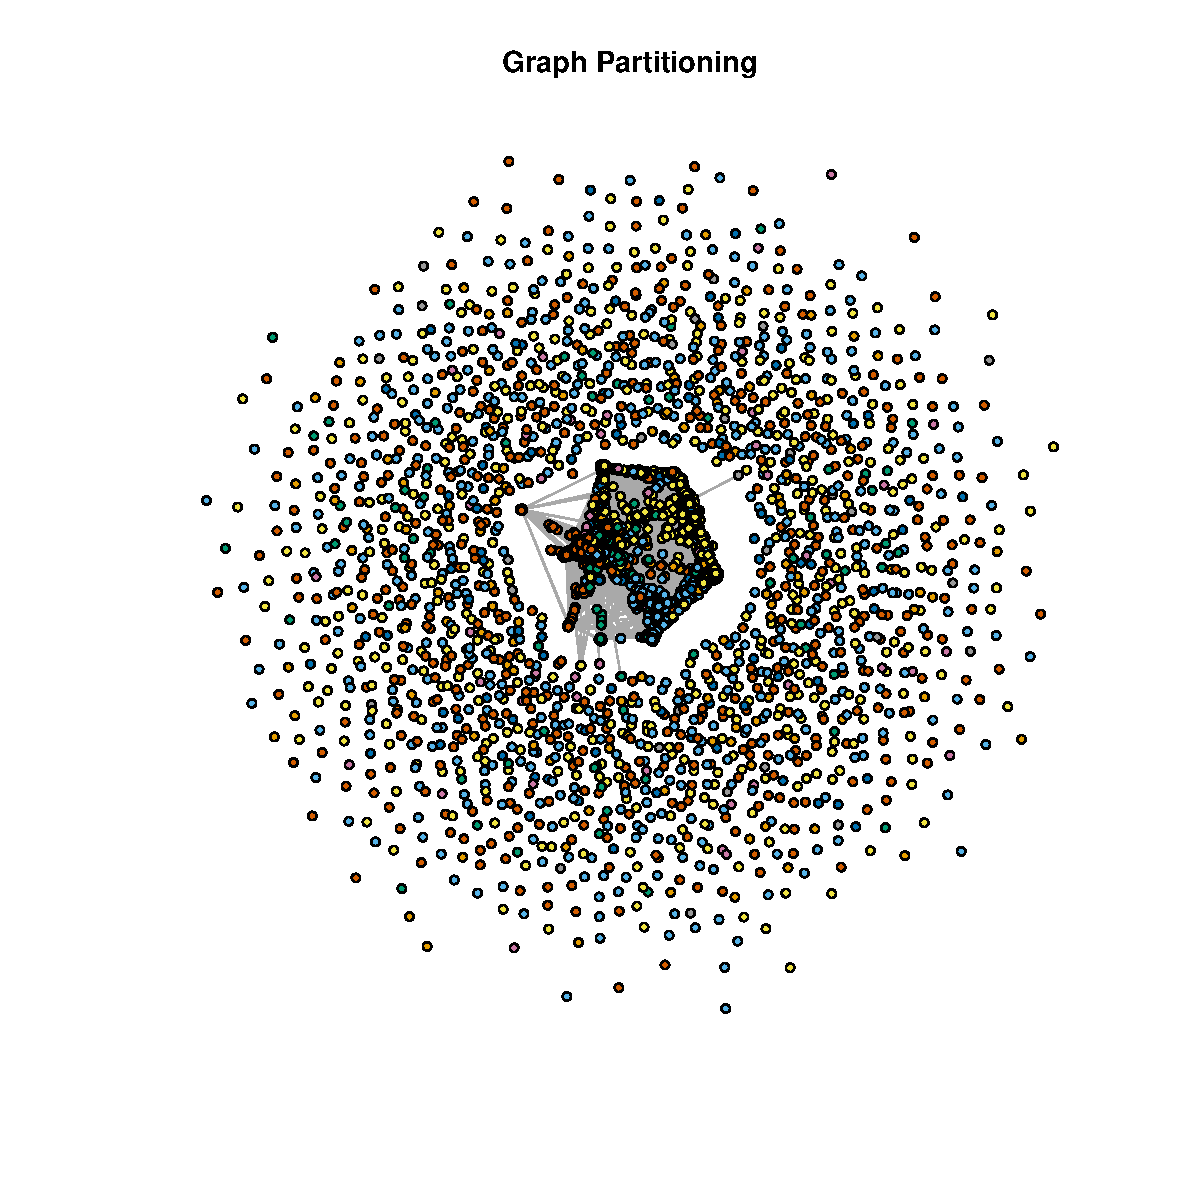
\includegraphics[width=0.8\textwidth]{output_plots/graph_partition.pdf}
  \caption{Graph partitioning of the GitHub network.}
  \label{fig:graph_partition}
\end{figure}
Structural partitioning using the Fast-Greedy Algorithm indicates that the network is centered on a single node, as confirmed by its modularity ($M = 0.3957$). The central cluster appears to function as a ``global hub'', to which the majority of the peripheral developers are connected.

A visual inspection of the partitioned graph suggests it is composed of distinct communities. Most striking is the presence of the main center community, where developers seem very closely connected, and most of the other developers are connected to it. To verify this, we plot the graph's $k$-core distribution.
\begin{figure}[H]
  \centering
  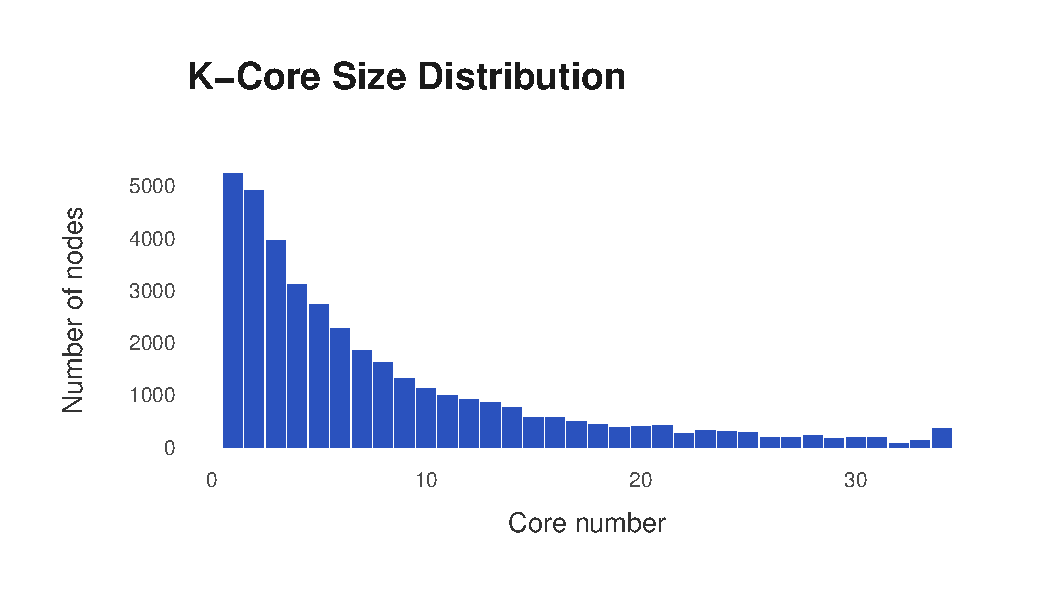
\includegraphics[width=0.8\textwidth]{output_plots/kcore_distribution.pdf}
  \caption{$K$-core distribution of the GitHub network}
  \label{fig:kcore_distribution}
\end{figure}
Looking at the $k$-core distribution, we see a large number of nodes in the first $k$-core, indicating they are very well connected to each other and appear to form the main community in the graph.

\begin{figure}[H]
  \centering
  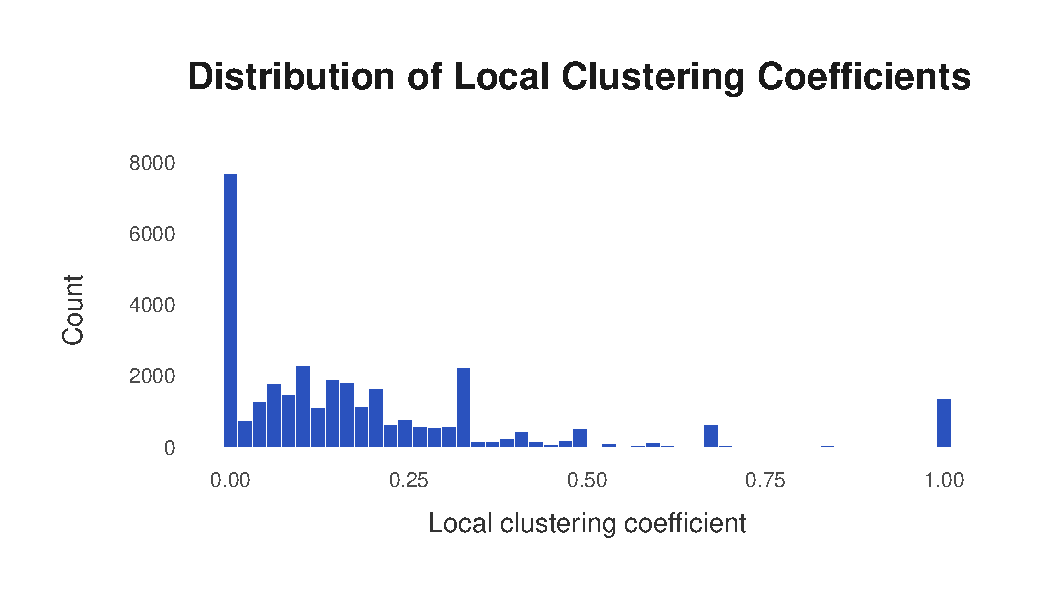
\includegraphics[width=0.8\textwidth]{output_plots/local_clustering.pdf}
  \caption{Local clustering of the GitHub network}
  \label{fig:local_clustering}
\end{figure}
As expected, the local clustering coefficient is quite low, indicating that this network indeed exhibits a hub-and-spoke structure. Also, the community size in the graph is quite important for understanding its structure.
\begin{table}[H]
  \centering
  \begin{tabular}{lr}
    \hline
    \textbf{Size} & \textbf{Count} \\
    \hline
    6  & 10,868 \\
    2  & 10,818 \\
    4  & 10,776 \\
    3  & 1,379  \\
    5  & 1,225  \\
    1  & 1,071  \\
    7  & 250    \\
    8  & 95     \\
    9  & 39     \\
    11 & 26     \\
    \hline
  \end{tabular}
  \caption{Top 10 Communities by Size using Fast-Greedy}
  \label{tab:community_sizes}
\end{table}
This is very interesting because it shows that many small communities exist in the graph, indicating that many developers are not connected to the main community but have their own smaller ones.

\subsection{Assortativity and Mixing Patterns}
Assortativity measures how likely it is for similar nodes to connect. We analyzed degree assortativity (whether popular developers tend to connect to other popular developers) and professional homophily (whether developers of the same type preferentially connect).
\begin{table}[H]
  \centering
  \begin{tabular}{lrl}
    \hline
    \textbf{Assortativity} & \textbf{Value} & \textbf{Interpretation} \\
    \hline
    Degree & $-0.075$ & Mildly disassortative (hubs connect to periphery) \\
    Job-type (homophily) & $+0.378$ & Strongly assortative (same type connects to same type) \\
    \hline
  \end{tabular}
  \caption{Assortativity coefficients}
  \label{tab:assortativity}
\end{table}

The negative degree coefficient ($r = -0.075$) indicates a hub-and-spoke pattern where high-degree developers attract followers from the broader pool of ordinary users rather than from other hubs. However, the strong positive professional coefficient ($r = 0.378$) indicates homophily: Machine Learning Engineers disproportionately follow other Machine Learning Engineers, and Web Developers follow other Web Developers. The mixing matrix quantifies this structure:

\begin{table}[H]
  \centering
  \begin{tabular}{l|rrr}
    \hline
    & \textbf{Web (0)} & \textbf{MLE (1)} & \textbf{Total} \\
    \hline
    \textbf{Web (0)} & 224,623 (77.7\%) & 44,696 (15.5\%) & 269,319 \\
    \textbf{MLE (1)} & 44,696 (15.5\%) & 19,684 (6.8\%) & 64,380 \\
    \hline
    \textbf{Total} & 269,319 & 64,380 & 289,003 \\
  \end{tabular}
  \caption{Edge mixing matrix by developer type. Each undirected edge is counted once; percentages show the fraction of total edges.}
  \label{tab:mixing}
\end{table}

However, this could be a base-rate artifact, since Web Developers outnumber Machine Learning Engineers roughly 3:1. To control for group size, we compute edge probabilities for each block pair (observed edges divided by the number of possible pairs).
\begin{table}[H]
  \centering
  \begin{tabular}{lrrr}
    \hline
    \textbf{Block Pair} & \textbf{Possible Pairs} & \textbf{Edge Count} & \textbf{Edge Prob.} \\
    \hline
    Web--Web & 390,894,780 & 224,623 & $5.75 \times 10^{-4}$ \\
    Web--MLE & 272,312,179 & 44,696 & $1.64 \times 10^{-4}$ \\
    MLE--MLE & 47,419,191 & 19,684 & $4.15 \times 10^{-4}$ \\
    \hline
  \end{tabular}
  \caption{Stochastic block model edge probabilities}
  \label{tab:sbm}
\end{table}

The within-group edge probabilities (Web--Web: $5.75 \times 10^{-4}$, MLE--MLE: $4.15 \times 10^{-4}$) exceed the cross-group probability ($1.64 \times 10^{-4}$) by $2.5$--$3.5\times$, which suggests that homophily is a genuine structural feature of the network.

\subsection{Comparison with Random Graph Models}
Random graphs allow researchers to analyze typical graph behaviors through probability without needing to map every node. To understand the behavior of the GitHub Network, we compare it against four classical random graph models. Each model preserves a specific property of the real network while randomizing the remaining structure, thereby serving as a controlled null hypothesis.

The first and simplest baseline is the \textbf{Erd\H{o}s--R{\'e}nyi} model, in which each of the $\binom{n}{2}$ possible edges exists independently with probability $p = 4.07 \times 10^{-4}$, matching the observed density; this preserves only the number of nodes and expected edge count. To account for the network's highly skewed degree distribution, we also consider the \textbf{Configuration Model}, which uniformly at random rewires edges while preserving the exact observed degree sequence, thereby isolating the contribution of degree heterogeneity from higher-order structural features. In addition, the \textbf{Watts--Strogatz} model \cite{watts1998smallworld} begins from a regular ring lattice in which each node is connected to its $k$ nearest neighbors and rewires edges with probability $p$, producing networks that exhibit high clustering and short average path lengths simultaneously. Finally, the \textbf{Barab{\'a}si--Albert} model grows the network incrementally via preferential attachment, where new nodes connect to existing nodes with probability proportional to current degree, yielding a power-law degree distribution.

\begin{table}[H]
  \centering
  \begin{tabular}{l|rrrrr}
    \hline
    \textbf{Model} & \textbf{Nodes} & \textbf{Mean Deg.} & \textbf{SD Deg.} & \textbf{Transitivity} & \textbf{Avg Path} \\
    \hline
    GitHub Network        & 37,700 & 15.33 & 80.79 & 0.0124 & 3.24 \\
    Erd\H{o}s--R{\'e}nyi & 37,700 & 15.33 & 3.92  & 0.0004 & 4.14 \\
    Configuration Model   & 37,700 & 15.33 & 80.79 & 0.0169 & 3.34 \\
    Watts--Strogatz       & 37,700 & 14.00 & 1.17  & 0.5052 & 4.25 \\
    Barab{\'a}si--Albert  & 37,700 & 16.00 & 19.88 & 0.0027 & 3.65 \\
    \hline
  \end{tabular}
  \caption{Comparison of network properties across random graph models}
  \label{tab:model_comparison}
\end{table}

\subsection{Small-World Assessment}
A network shows a small-world structure \cite{watts1998smallworld} if it has substantially higher clustering but the same average path length as a comparable random graph. This is quantified with the small-world score $\sigma = (C_{\text{obs}}/C_{\text{ER}}) / (L_{\text{obs}}/L_{\text{ER}})$, where $\sigma \gg 1$ means small-world structure.

\begin{table}[H]
  \centering
  \begin{tabular}{l|rrr}
    \hline
    \textbf{Property} & \textbf{GitHub} & \textbf{ER Mean} & \textbf{Ratio} \\
    \hline
    Clustering coeff.\ $C$ & 0.0124 & 0.000409 & $30.2$ \\
    Avg.\ path length $L$ & 3.24 & 4.13 & $0.78$ \\
    \hline
  \end{tabular}
  \caption{Comparison between GitHub network and Erd\H{o}s--R{\'e}nyi}
  \label{tab:smallworld}
\end{table}

Here, the small-world score is $\sigma = 30.2 / 0.78 \approx 38.7 \gg 1$, which means that this GitHub network exhibits small-world structure. This means that any developer can reach another developer on average through 3 to 4 connectors, but their neighborhoods are 30 times more connected, indicating a tight-knit structure.

\section{Results}
The graph is a \textbf{undirected}, \textbf{simple}, and \textbf{globally connected}, \textbf{sparse} graph with high local connectivity. The degree distribution follows a power-law tail indicating a "winner-take-all" dynamic because of a small elite of "Hub" nodes. The network follows a small-world scenario because of substantially high clustering coefficient compared to a random Erdos-Renyi graph despite similar path lengths. Lastly, the network shows a mild negative degree assortavity but very strong professional homophily.

\section{Discussion}
The GitHub Network shows some vulnerabilities to the `gatekeeper' developers. Because there are only 350 articulation points for over 37,000 developers, removing one of those key hubs would fragment the global open-source community into isolated clusters. Secondly, because the network shows a significant professional homophily, the developers might preferentially follow their fellow developers leading to a situation of echo chambers because of lack of interaction between the other type of developers. Third, GitHub network follows the \underline{Barabasi-Albert} random graph model closely, which shows that new users are disproportionately following already established developers which shows the popularity of \textit{addyosmani} and \textit{jeresig}.
\section{Future Work}
This project could be significantly improved with the use of more recent data such as 2025 and onwards. With the rise of Large Language Models, Machine Learning noticed a significant propfessional and economic growth, and simultaneously, Large Language Models have gotten significantly better than entry-level web developers so there is a change which should be studied. Additionally, link prediction is also quite important because it would provide insights into how the community grows, functions and sustains itself. Subsequently, because of computational intensity, higher order models like Exponential Random Models were not used. In future, implementing ERGMs would give more information about the graph.
Link Prediction
\nocite{*}
\bibliographystyle{plain}
\bibliography{lib}
% Ego Network – take a very well-connected node, find its ego networks, and plot that
% Sasha's Clustering is also very good. I think I might want to include that in my plot.
\end{document}